\documentclass[border={8pt 8pt 8pt 14pt}]{standalone}
\usepackage{tikz}
\usetikzlibrary{arrows.meta, positioning, calc, fit, backgrounds}
\begin{document}
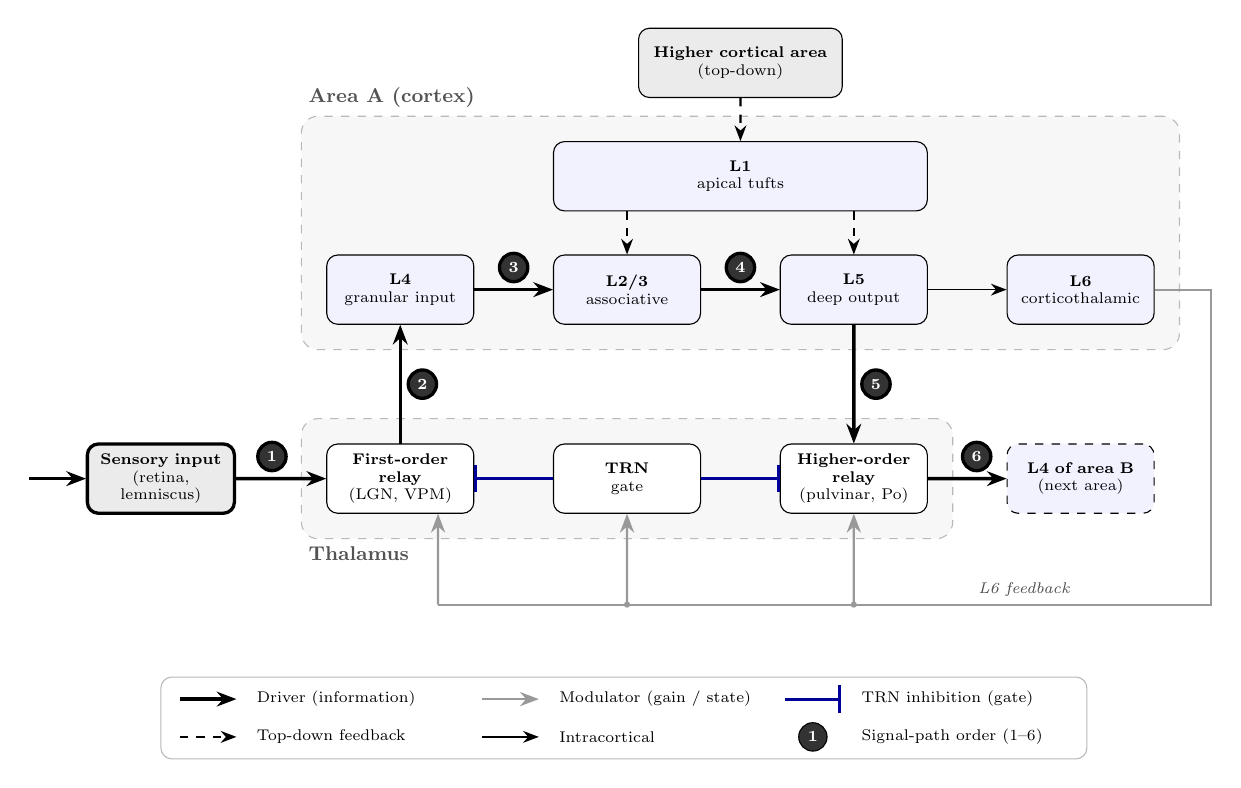
\begin{tikzpicture}[
  scale=0.8, transform shape,
  box/.style={draw, rectangle, rounded corners, minimum height=1.1cm,
              text width=2.1cm, align=center, font=\scriptsize},
  col/.style={box, fill=blue!5},                 % cortex
  thn/.style={box, fill=white},                  % thalamic nuclei (region carries the grouping)
  ext/.style={box, fill=black!8},                % external: periphery / other areas
  entry/.style={ext, line width=1.2pt},          % start of the flow
  driver/.style={-{Stealth[length=2.5mm]}, line width=1.2pt},
  intra/.style={-{Stealth[length=2mm]}, line width=0.6pt},
  modulator/.style={-{Stealth[length=2.4mm]}, line width=0.8pt, draw=gray!80},
  modline/.style={line width=0.8pt, draw=gray!80},
  gate/.style={-{Bar[width=3.5mm]}, line width=1.1pt, draw=blue!60!black},
  topdown/.style={-{Stealth[length=2mm]}, line width=0.8pt, dashed},
  bignum/.style={circle, draw, fill=black!80, text=white,
                 font=\scriptsize\bfseries, minimum size=4.5mm, inner sep=0pt},
  region/.style={draw=gray!55, dashed, rounded corners=6pt,
                 fill=gray!6, inner sep=9pt},
  regionlabel/.style={font=\small\bfseries, text=gray!65!black},
  legtext/.style={font=\scriptsize, anchor=west},
]
  % ---- Cortical column (area A), left to right: L4 -> L2/3 -> L5 -> L6 ----
  \node[col] (l4)  at (0,0)    {\textbf{L4}\\granular input};
  \node[col] (l23) at (3.6,0)  {\textbf{L2/3}\\associative};
  \node[col] (l5)  at (7.2,0)  {\textbf{L5}\\deep output};
  \node[col] (l6)  at (10.8,0) {\textbf{L6}\\corticothalamic};
  % L1 spans above L2/3 and L5 (apical tufts of their pyramids)
  \node[col, text width=5.7cm] (l1) at (5.4,1.8) {\textbf{L1}\\apical tufts};

  % ---- Top-down source, directly above L1 ----
  \node[ext, text width=3cm] (hi) at (5.4,3.6) {\textbf{Higher cortical area}\\(top-down)};

  % ---- Thalamus: FO relay under L4, TRN between relays, HO relay under L5 ----
  \node[thn] (fo)  at (0,-3)   {\textbf{First-order}\\\textbf{relay}\\(LGN, VPM)};
  \node[thn] (trn) at (3.6,-3) {\textbf{TRN}\\gate};
  \node[thn] (ho)  at (7.2,-3) {\textbf{Higher-order}\\\textbf{relay}\\(pulvinar, Po)};

  % ---- External nodes ----
  \node[entry] (sens) at (-3.8,-3) {\textbf{Sensory input}\\(retina, lemniscus)};
  \node[col, dashed] (b) at (10.8,-3) {\textbf{L4 of area B}\\(next area)};

  % ---- Regions (drawn behind everything) ----
  \begin{scope}[on background layer]
    \node[region, fit=(l1)(l4)(l23)(l5)(l6)] (ctxA) {};
    \node[region, fit=(fo)(trn)(ho)] (thal) {};
  \end{scope}
  \node[regionlabel, anchor=south west] at (ctxA.north west) {Area A (cortex)};
  \node[regionlabel, anchor=north west] at (thal.south west) {Thalamus};

  % ==== ENTRY STUB ====
  \draw[driver] ([xshift=-9mm]sens.west) -- (sens.west);

  % ==== DRIVER PATH (numbered 1-6, thick) ====
  \draw[driver] (sens) -- node[bignum, above=3pt, pos=0.4]  {1} (fo);   % sensory -> FO relay
  \draw[driver] (fo)   -- node[bignum, right=3pt]           {2} (l4);   % FO relay -> L4 (ascending)
  \draw[driver] (l4)   -- node[bignum, above=3pt]           {3} (l23);  % L4 -> L2/3
  \draw[driver] (l23)  -- node[bignum, above=3pt]           {4} (l5);   % L2/3 -> L5
  \draw[driver] (l5)   -- node[bignum, right=3pt]           {5} (ho);   % L5 -> HO relay (output)
  \draw[driver] (ho)   -- node[bignum, above=3pt, pos=0.62] {6} (b);    % HO relay -> area B

  % ==== Intracortical (not part of the driver path, no badge) ====
  \draw[intra] (l5) -- (l6);                                            % L5 -> L6

  % ==== TOP-DOWN FEEDBACK (dashed) ====
  \draw[topdown] (hi) -- (l1);                                          % higher area -> L1
  \draw[topdown] (l1.south -| l23) -- (l23.north);                      % L1 tufts -> L2/3
  \draw[topdown] (l1.south -| l5)  -- (l5.north);                       % L1 tufts -> L5

  % ==== L6 MODULATORY FEEDBACK (thin grey) ====
  % trunk: east of L6, down past area B, west under the Thalamus label
  \draw[modline] (l6.east) -- ++(0.9,0) |- (0.6,-5);
  \node[font=\scriptsize\itshape, text=gray!60!black, above] at (9.9,-5) {L6 feedback};
  % branches up into the thalamus
  \draw[modulator] (0.6,-5) -- ([xshift=6mm]fo.south);                  % L6 -> FO relay
  \draw[modulator] (3.6,-5) -- (trn.south);                             % L6 -> TRN
  \draw[modulator] (7.2,-5) -- (ho.south);                              % L6 -> HO relay
  \fill[gray!80] (3.6,-5) circle (1.4pt);
  \fill[gray!80] (7.2,-5) circle (1.4pt);

  % ==== TRN GATE (inhibitory, bar-ended) ====
  \draw[gate] (trn.west) -- (fo.east);                                  % TRN -| FO relay
  \draw[gate] (trn.east) -- (ho.west);                                  % TRN -| HO relay

  % ==== LEGEND (Stage 4) ====
   % ==== LEGEND (Stage 4) ====
  \begin{scope}[shift={(-2,-6.5)}]
    % row 1
    \draw[driver]    (-1.5,0) -- (-0.6,0);
    \node[legtext] at (-0.4,0) {Driver (information)};
    \draw[modulator] (3.3,0)  -- (4.2,0);
    \node[legtext] at (4.4,0)  {Modulator (gain / state)};
    \draw[gate]      (8.1,0)  -- (9.0,0);
    \node[legtext] at (9.2,0)  {TRN inhibition (gate)};
    % row 2
    \draw[topdown]   (-1.5,-0.6) -- (-0.6,-0.6);
    \node[legtext] at (-0.4,-0.6) {Top-down feedback};
    \draw[intra]     (3.3,-0.6)  -- (4.2,-0.6);
    \node[legtext] at (4.4,-0.6)  {Intracortical};
    \node[bignum]  at (8.55,-0.6) {1};
    \node[legtext] at (9.2,-0.6)  {Signal-path order (1--6)};
    % frame
    \draw[gray!55, rounded corners=4pt] (-1.8,0.35) rectangle (12.9,-0.95);
  \end{scope}
\end{tikzpicture}
\end{document}